\documentclass[tikz, border=10pt]{standalone}
\usepackage{amsmath}
\usepackage{tikz}
\usetikzlibrary{decorations.pathmorphing, arrows.meta, calc, backgrounds}

\definecolor{navybg}{RGB}{13,27,42}
\definecolor{source1col}{RGB}{0,220,255}
\definecolor{source2col}{RGB}{255,165,0}
\definecolor{wavecol}{RGB}{255,215,0}
\definecolor{starglow}{RGB}{255,255,200}
\definecolor{labelcol}{RGB}{220,220,220}
\definecolor{plotbg}{RGB}{25,40,60}

\begin{document}
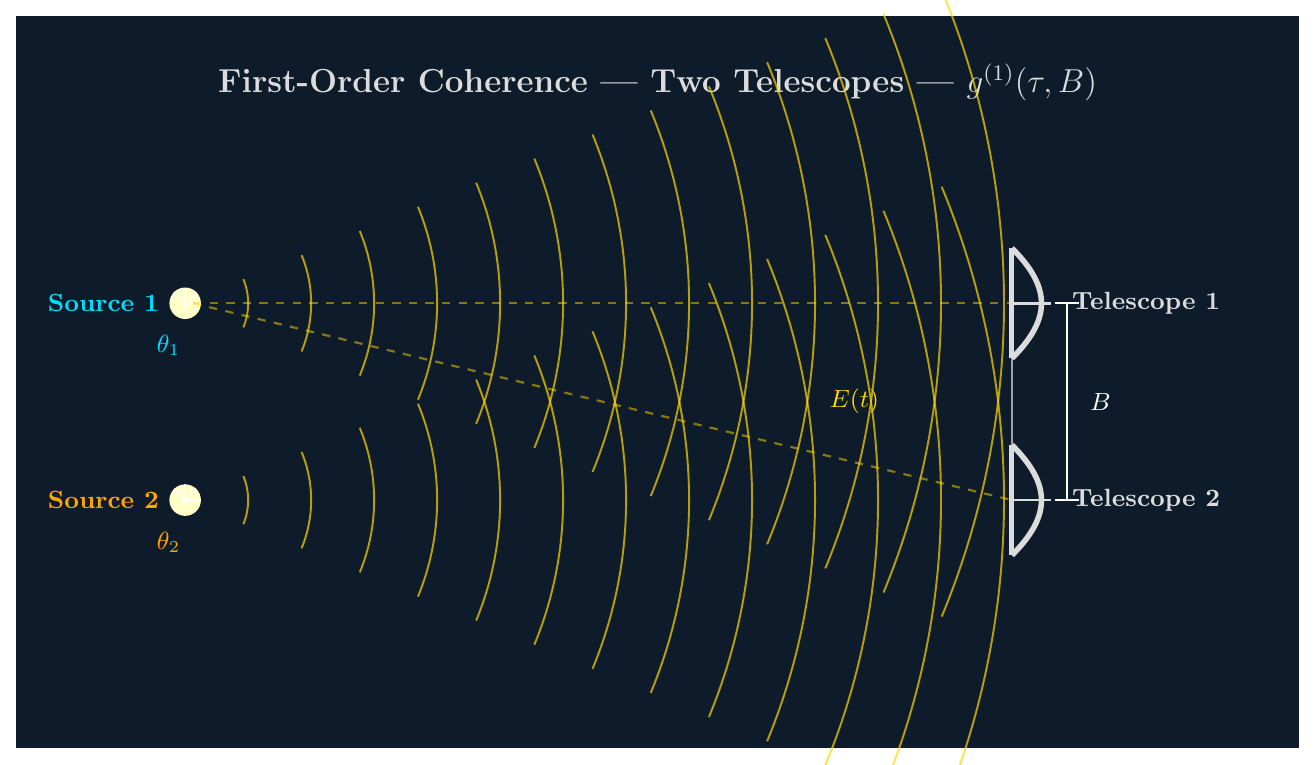
\begin{tikzpicture}[
    background rectangle/.style={fill=navybg},
    show background rectangle,
    wave/.style={decorate,
                 decoration={snake, amplitude=2.5pt, segment length=7pt}},
]

\path[use as bounding box] (0,0) rectangle (16,9);

% ════════════════════════════════════════════════════════
% 0. TITLE
% ════════════════════════════════════════════════════════
\node[text=labelcol, font=\large\bfseries] at (8.0, 8.3)
    {First-Order Coherence \textemdash\ Two Telescopes
     \textemdash\ $g^{(1)}(\tau,B)$};

% ════════════════════════════════════════════════════════
% 1. TWO POINT SOURCES (LEFT SIDE)
% ════════════════════════════════════════════════════════
\coordinate (S1) at (2.0, 5.5);
\coordinate (S2) at (2.0, 3.0);

% Glow halos S1
\foreach \r/\op in {0.20/15, 0.12/30, 0.06/60}{
    \fill[starglow, opacity=\op] (S1) circle (\r);
}
\fill[white] (S1) circle (0.04);
\foreach \ang in {0,45,90,135}{
    \draw[white, line width=0.6pt, opacity=0.8]
        ($(S1)+(\ang:0.06)$) -- ($(S1)+(\ang:0.20)$);
}
\node[text=source1col, font=\small\bfseries, left=6pt] at (S1) {Source 1};

% Glow halos S2
\foreach \r/\op in {0.20/15, 0.12/30, 0.06/60}{
    \fill[starglow, opacity=\op] (S2) circle (\r);
}
\fill[white] (S2) circle (0.04);
\foreach \ang in {0,45,90,135}{
    \draw[white, line width=0.6pt, opacity=0.8]
        ($(S2)+(\ang:0.06)$) -- ($(S2)+(\ang:0.20)$);
}
\node[text=source2col, font=\small\bfseries, left=6pt] at (S2) {Source 2};

% Absolute angular positions — one label per source, below source labels
\node[text=source1col, font=\small, left=6pt, below=8pt] at (S1) {$\theta_1$};
\node[text=source2col, font=\small, left=6pt, below=8pt] at (S2) {$\theta_2$};

% ════════════════════════════════════════════════════════
% 2. ELECTRIC FIELD WAVEFRONTS FROM SOURCES
%    Concentric arcs around each source
% ════════════════════════════════════════════════════════
\coordinate (TEL1) at (12.5, 5.5);
\coordinate (TEL2) at (12.5, 3.0);

% ── Concentric arcs from S1 (toward telescope) ────────
\draw[wavecol, line width=0.7pt, opacity=0.7]
    ($(S1) + ({0.8*cos(-22.5)}, {0.8*sin(-22.5)})$) arc(-22.5:22.5:0.8);
\draw[wavecol, line width=0.7pt, opacity=0.7]
    ($(S1) + ({1.6*cos(-22.5)}, {1.6*sin(-22.5)})$) arc(-22.5:22.5:1.6);
\draw[wavecol, line width=0.7pt, opacity=0.7]
    ($(S1) + ({2.4*cos(-22.5)}, {2.4*sin(-22.5)})$) arc(-22.5:22.5:2.4);
\draw[wavecol, line width=0.7pt, opacity=0.7]
    ($(S1) + ({3.2*cos(-22.5)}, {3.2*sin(-22.5)})$) arc(-22.5:22.5:3.2);
\draw[wavecol, line width=0.7pt, opacity=0.7]
    ($(S1) + ({4.0*cos(-22.5)}, {4.0*sin(-22.5)})$) arc(-22.5:22.5:4.0);
\draw[wavecol, line width=0.7pt, opacity=0.7]
    ($(S1) + ({4.8*cos(-22.5)}, {4.8*sin(-22.5)})$) arc(-22.5:22.5:4.8);
\draw[wavecol, line width=0.7pt, opacity=0.7]
    ($(S1) + ({5.6*cos(-22.5)}, {5.6*sin(-22.5)})$) arc(-22.5:22.5:5.6);
\draw[wavecol, line width=0.7pt, opacity=0.7]
    ($(S1) + ({6.4*cos(-22.5)}, {6.4*sin(-22.5)})$) arc(-22.5:22.5:6.4);
\draw[wavecol, line width=0.7pt, opacity=0.7]
    ($(S1) + ({7.2*cos(-22.5)}, {7.2*sin(-22.5)})$) arc(-22.5:22.5:7.2);
\draw[wavecol, line width=0.7pt, opacity=0.7]
    ($(S1) + ({8.0*cos(-22.5)}, {8.0*sin(-22.5)})$) arc(-22.5:22.5:8.0);
\draw[wavecol, line width=0.7pt, opacity=0.7]
    ($(S1) + ({8.8*cos(-22.5)}, {8.8*sin(-22.5)})$) arc(-22.5:22.5:8.8);
\draw[wavecol, line width=0.7pt, opacity=0.7]
    ($(S1) + ({9.6*cos(-22.5)}, {9.6*sin(-22.5)})$) arc(-22.5:22.5:9.6);
\draw[wavecol, line width=0.7pt, opacity=0.7]
    ($(S1) + ({10.4*cos(-22.5)}, {10.4*sin(-22.5)})$) arc(-22.5:22.5:10.4);

% ── Concentric arcs from S2 (toward telescope) ────────
\draw[wavecol, line width=0.7pt, opacity=0.7]
    ($(S2) + ({0.8*cos(-22.5)}, {0.8*sin(-22.5)})$) arc(-22.5:22.5:0.8);
\draw[wavecol, line width=0.7pt, opacity=0.7]
    ($(S2) + ({1.6*cos(-22.5)}, {1.6*sin(-22.5)})$) arc(-22.5:22.5:1.6);
\draw[wavecol, line width=0.7pt, opacity=0.7]
    ($(S2) + ({2.4*cos(-22.5)}, {2.4*sin(-22.5)})$) arc(-22.5:22.5:2.4);
\draw[wavecol, line width=0.7pt, opacity=0.7]
    ($(S2) + ({3.2*cos(-22.5)}, {3.2*sin(-22.5)})$) arc(-22.5:22.5:3.2);
\draw[wavecol, line width=0.7pt, opacity=0.7]
    ($(S2) + ({4.0*cos(-22.5)}, {4.0*sin(-22.5)})$) arc(-22.5:22.5:4.0);
\draw[wavecol, line width=0.7pt, opacity=0.7]
    ($(S2) + ({4.8*cos(-22.5)}, {4.8*sin(-22.5)})$) arc(-22.5:22.5:4.8);
\draw[wavecol, line width=0.7pt, opacity=0.7]
    ($(S2) + ({5.6*cos(-22.5)}, {5.6*sin(-22.5)})$) arc(-22.5:22.5:5.6);
\draw[wavecol, line width=0.7pt, opacity=0.7]
    ($(S2) + ({6.4*cos(-22.5)}, {6.4*sin(-22.5)})$) arc(-22.5:22.5:6.4);
\draw[wavecol, line width=0.7pt, opacity=0.7]
    ($(S2) + ({7.2*cos(-22.5)}, {7.2*sin(-22.5)})$) arc(-22.5:22.5:7.2);
\draw[wavecol, line width=0.7pt, opacity=0.7]
    ($(S2) + ({8.0*cos(-22.5)}, {8.0*sin(-22.5)})$) arc(-22.5:22.5:8.0);
\draw[wavecol, line width=0.7pt, opacity=0.7]
    ($(S2) + ({8.8*cos(-22.5)}, {8.8*sin(-22.5)})$) arc(-22.5:22.5:8.8);
\draw[wavecol, line width=0.7pt, opacity=0.7]
    ($(S2) + ({9.6*cos(-22.5)}, {9.6*sin(-22.5)})$) arc(-22.5:22.5:9.6);
\draw[wavecol, line width=0.7pt, opacity=0.7]
    ($(S2) + ({10.4*cos(-22.5)}, {10.4*sin(-22.5)})$) arc(-22.5:22.5:10.4);

% ── E(t) label for wavefront ────────────────────────
\node[text=wavecol, font=\small] at (10.5, 4.25) {$E(t)$};

% ════════════════════════════════════════════════════════
% 2b. PATH DELAY VISUALIZATION
%     Show geometric path difference from sources to telescopes
% ════════════════════════════════════════════════════════
% Dashed wavefront from S1 to TEL1 (shorter path)
\draw[wavecol, line width=0.8pt, opacity=0.5, dashed]
    ($(S1)+(0.1, 0)$) -- ($(TEL1)+(0.0, 0.0)$);

% Dashed wavefront from S1 to TEL2 (longer path due to tilt)
\draw[wavecol, line width=0.8pt, opacity=0.5, dashed]
    ($(S1)+(0.1, 0)$) -- ($(TEL2)+(0.0, 0.0)$);

% Path difference indicator arc
\draw[white, line width=0.6pt, opacity=0.6]
    ($(TEL1)+(0.0, -0.5)$) -- ($(TEL2)+(0.0, -0.5)$);
\node[text=white, font=\small, below=3pt] at (12.5, -0.5) {$\Delta \tau = \frac{B \sin \theta_s}{c}$};

% ════════════════════════════════════════════════════════
% 3. TWO TELESCOPES (RIGHT SIDE, facing left)
% ════════════════════════════════════════════════════════
% Telescope 1 (upper)
\draw[labelcol, line width=2pt]
    ($(TEL1)+(0.0,  0.7)$)
    .. controls ($(TEL1)+(0.5, 0.2)$) and ($(TEL1)+(0.5,-0.2)$) ..
    ($(TEL1)+(0.0, -0.7)$);
\draw[labelcol, line width=1.8pt]
    ($(TEL1)+(0.0, 0.7)$) -- ($(TEL1)+(0.0,-0.7)$);
\draw[labelcol, line width=1.0pt]
    ($(TEL1)+(0.0, 0.0)$) -- ($(TEL1)+(0.5, 0.0)$);

\node[text=labelcol, font=\small\bfseries, right=4pt]
    at ($(TEL1)+(0.5, 0.0)$) {Telescope 1};

% Telescope 2 (lower)
\draw[labelcol, line width=2pt]
    ($(TEL2)+(0.0,  0.7)$)
    .. controls ($(TEL2)+(0.5, 0.2)$) and ($(TEL2)+(0.5,-0.2)$) ..
    ($(TEL2)+(0.0, -0.7)$);
\draw[labelcol, line width=1.8pt]
    ($(TEL2)+(0.0, 0.7)$) -- ($(TEL2)+(0.0,-0.7)$);
\draw[labelcol, line width=1.0pt]
    ($(TEL2)+(0.0, 0.0)$) -- ($(TEL2)+(0.5, 0.0)$);

\node[text=labelcol, font=\small\bfseries, right=4pt]
    at ($(TEL2)+(0.5, 0.0)$) {Telescope 2};

% Baseline B
\draw[white, line width=0.8pt]
    ($(TEL1)+(0.7, 0.0)$) -- ($(TEL2)+(0.7, 0.0)$);
\draw[white, line width=0.6pt]
    ($(TEL1)+(0.55, 0.0)$) -- ($(TEL1)+(0.85, 0.0)$);
\draw[white, line width=0.6pt]
    ($(TEL2)+(0.55, 0.0)$) -- ($(TEL2)+(0.85, 0.0)$);
\node[text=white, font=\small, right=2pt] at (13.3, 4.25) {$B$};

\end{tikzpicture}
\end{document}
